\section{Desenvolvimento realizado na empresa}
\label{sec:desenvolvimento}

{Nesta sessão será apresentada a ferramenta desenvolvida como solução ao problema de acessibilidade em e-commerce no CESAR, abordando as técnicas, tecnologias utilizadas e contribuições para a empresa.}

\subsection{A problemática e a solução proposta}
{A construção de um e-commerce com um painel administrativo composto por um dashboard aplicando diretrizes de acessibilidade, usabilidade e boas práticas. Tornando possível o uso do e-commerce por pessoas com deficiências visuais. 

Assim que foi definida a temática do trabalho, o primeiro passo foi solicitar autorização à gerência e setores para realizá-lo, deixando claro todos os cuidados que seriam tomados com as informações e também os ganhos para o negócio.}

\subsection{Fase 1: Pesquisa e entendimento}
{A construção do e-commerce ocorreu em 4 fases, sendo a primeira fase voltada para o entendimento do problema e do uso das novas tecnologias como também entender as limitações do projeto em questão de performance e se seria possível ou não adicionar novas bibliotecas caso fosse necessário. Ainda na primeira fase, após concluída a fase de estudo e exploração o time optou por construir um guia de acessibilidade que seria usado na fase de desenvolvimento do projeto, essa decisão se deu porque a documentação das diretrizes de acessibilidade é bastante extensa e engloba muitos tipos de deficiência, sendo assim tornando-se de difícil entendimento para todos que estão lendo. Para complementar o guia de acessibilidade foi construído um style guide para guiar todos os desenvolvedores a respeito de aspectos importantes de uma UI como  comportamento de componentes e cores acessíveis}

\subsubsection{Guia de acessibilidade}
{Quando falamos em acessibilidade precisamos citar o WCAG ou Web Content Accessibility Guidelines é um documento que estipula os padrões de acessibilidade digital que devem ser seguidos pelos sites. Essas recomendações foram todas desenvolvidas pelo W3C, o consórcio World Wide Web.

O WCAG é responsável por orientar de forma muito simples como identificar e implementar técnicas que eliminam barreiras de acesso para pessoas com deficiência e ele foi construído sob quatro princípios:
\begin{itemize}
\item Perceptível: As informações e os componentes da interface do usuário devem ser apresentados de formas que possam ser percebidas pelo usuário.
\item Operável: Os componentes da interface de usuário e a navegação devem ser operáveis. O usuário não pode ter impedimentos para utilizar a interface.
\item Compreensível: A informação e a operação da interface de usuário devem ser compreensíveis. 
\item Robusto: O conteúdo deve ser robusto o suficiente para poder ser interpretado de forma confiável por uma ampla variedade de agentes de usuário, incluindo tecnologias assistivas. a aplicação deve ser bem construída, de forma a ser acessível para uma gama maior de navegadores e tecnologias assistiva
\end{itemize}

Guiado por esses quatro princípios surgiram as diretrizes, que são os itens que fornecem os objetivos básicos que devem ser atingidos dentro de cada principio, que são tópicos menores e mais específicos. Dentro das diretrizes existe critérios de sucesso, esse sucesso está atrelado a nível de conformidade. Então quanto mais conforme o e-commerce está adequado à aquela diretriz maior é o critério de sucesso. Os critérios são definidos três níveis de conformidade:
\begin{itemize}
\item No nível A estão os critérios mais simples, que representam apenas barreiras mais significativas de acessibilidade. Ao obter sucesso nesse critério já é possível eliminar uma boa quantidade de barreiras de acesso. 
\item No nível AA,  apresenta para a maior parte dos usuários, garantindo acesso à grande maioria dos conteúdos, os critérios do nível A geralmente já foram obtidos quando você obtém sucesso nos critérios de nível AA.
\item Nível AAA, geralmente são um refinamento das anteriores, sendo mais detalhadas e que trazem um nível mais sofisticado de acessibilidade.
\end{itemize}

Dentre todas as diretrizes WCAG que existem foram escolhidas algumas que fizessem sentido no contexto de diminuição de barreiras de acesso para deficientes visuais. Toda a construção do e-commerce foi baseada nessas diretrizes abaixo: 
\begin{itemize}
\item 1.1.1 - Conteúdo não Textual [A]: Todo conteúdo "não textual" e relevante para compreensão da informação, deve trazer uma descrição alternativa em texto para identificar o conteúdo.
\item 1.3.1 - Informações e Relações [A]: As estruturas da tela devem ser construída de forma que sua arquitetura de informação faça sentido tanto para todos, sejam ouvintes ou leitores.
\item 1.3.2 - Sequência com significado [A]: A apresentação das informações na tela sempre deverá ter uma sequência lógica.
\item 1.3.5 - Identificar o objetivo de entrada [AA]: Deve ser claro para as pessoas o que deve ser preenchido em campos de formulários.
\item 1.4.1 - Utilização de cores [A]: As cores não devem carregar significado lógico, elas não devem ser utilizadas como única maneira de transmitir conteúdo ou distinguir elementos visuais.
\item 1.4.3 - Contraste (mínimo) [AA]: Textos devem ter uma relação de contraste entre primeiro e segundo plano de ao menos 4.5:1.
\item 1.4.4 - Redimensionar texto [AA]: Ao se aplicar zoom de até 200 \% na tela, deve ocorrer a responsividade dos textos apresentados de forma que sua leitura e legibilidade continuem adequados sem qualquer quebra na apresentação das informações.
\item 1.4.6 - Contraste (melhorado) [AAA]: Textos devem ter uma relação de contraste entre primeiro e segundo plano de ao menos 7:1.
\item 1.4.11 - Contraste Não-Textual [AA]: Componentes de interface e imagens essenciais para o entendimento do conteúdo devem ter uma relação de contraste entre primeiro e segundo plano de ao menos 3:1.
\item 1.4.12 - Espaçamento de texto [AA]: Sempre que houver um redimensionamento os textos não devem perder legibilidade.
\item 1.4.13 - Conteúdo em foco por mouse ou teclado [AA]: Conteúdos adicionais não devem ser acionados apenas com foco por mouse ou teclado. 
\item 2.1.1 - Teclado [A]: Todas as funcionalidades devem ser acionadas via teclado, com exceção se a funcionalidade não possibilite o controle apenas por teclado.
\item 2.1.2 - Sem bloqueio de teclado [A]: Ao se interagir via teclado, a navegação por todos os elementos "clicáveis" deve ocorrer sem que haja bloqueios ou interrupções.
\item 2.1.3 - Teclado (sem exceção) [AAA]: Todas as funcionalidades devem ser acionadas via teclado, sem exceção.
\item 2.2.3 - Sem limite de tempo [AAA]: Nenhuma funcionalidade em tela deve possuir algum tipo de execução mediante o cumprimento em um determinado período de tempo.
\item 2.2.4 - Interrupções [AAA]: Deve ser possível adiar os desligar qualquer tipo de interrupção acionada no sistema.
\item 2.2.5 - Nova autenticação [AAA]: Quando uma sessão autenticada expira, o usuário deve ser capaz de continuar sua atividade sem que haja perca de dados até que seja feita um nova autenticação.
\item 2.4.1 - Ignorar blocos [A]: Deve ser fornecido um tipo de controle para que as pessoas possam ignorar determinados conteúdos repetitivos e assim continuar com a navegação.
\item 2.4.2 - Página com título [A]: Todas as telas devem ter um título principal e que descreva claramente a sua finalidade.
\item 2.4.3 - Ordem do foco [A]: A interação por elementos focáveis na tela sempre deverá ser sequencial e lógica de acordo com o conteúdo apresentado.
\item 2.4.4 - Finalidade do link (em contexto) [A]: A finalidade de um link deve ser determinada a partir do texto do próprio link ou a partir do contexto no entorno deste link.
\begin{itemize}
\item 2.4.9 - Finalidade do link (apenas link) [AAA]: A finalidade de um link deve ser determinada a partir do texto do próprio link.
\end{itemize}
\item 2.4.5 - Várias formas [AA]: Deve ser fornecido mais de uma forma de as pessoas encontrarem um determinado conteúdo. 
\item 2.4.6 - Cabeçalhos e rótulos [AA]: Todos os títulos e rótulo devem descrever claramente a finalidade dos conteúdos, não deve haver ambiguidade em seu entendimento.
\begin{itemize}
\item 2.4.10 - Cabeçalhos da seção [AAA]: Sempre que o conteúdo da tela for dividido em sessões, todas devem possuir títulos claros, com níveis de hierarquia bem definidos, facilitando a identificação das áreas.
\end{itemize}
\item 2.4.7 - Foco visível [A]: Ao se interagir por teclado, qualquer pessoa deve conseguir identificar qual é a sua localização espacial na tela através de um foco visível identificador de sua localização.
\item 2.4.8 - Localização [AAA]: Qualquer pessoa deve conseguir se localizar ou se orientar facilmente em qualquer nas telas.
\item 2.5.2 - Cancelamento de acionamento[A]: Deve se fornecer um modo de cancelar acionamentos feitos de forma não proposital.
\item 2.5.3 - Rótulo no Nome acessível [A]: Rótulos em botões, ícones acionáveis ou qualquer controle interativo, devem ter uma descrição significativa.
\item 2.5.5 - Tamanho da área clicável [AAA]: O tamanho das áreas acionáveis por clique ou toque devem possuir no mínimo 44x44 pixeis de espaçamento, a não ser quando essa área esteja em uma frase localizada em um bloco de texto.
\item 3.1.1 - Idioma da página [A]: Declarar adequadamente o idioma da tela faz com que leitores de telas utilizem uma entonação correta para citar conteúdos. Sempre os declare.
\begin{itemize}
\item 3.1.2 - Idioma das partes [AA]: O idioma de uma determinada palavra ou frase contendo idioma diferente do original da tela, deve ser definido e corretamente identificado para que também ocorra uma correta entonação e pronúncia adequada via leitores de tela.
\item 3.1.3 - Palavras incomuns [AAA]: O uso de gírias, jargões, metáforas e figuras de linguagem pode ser um empecilho para a compreensão da informação, nesse sentido deve-se fornecer uma forma de tradução ou explicação da informação.
\end{itemize}
\item 3.1.4 - Abreviações [AAA]: Nem sempre uma abreviação ou um acrônimo é compreensível por todas as pessoas, nesse sentido deve-se fornecer uma forma de identificação de seu significado real (exemplo: link para acessar uma tabela de "de-para").
\item 3.1.6 - Pronúncia [AAA]: Palavras regionais específicas e nomes próprios costumam ter pronúncias também específicas. Deve ser fornecida uma forma de possibilitar a correta compreensão da pronúncia em alguns casos.
\item 3.2.1 - Em foco [A]: O foco sempre deve se manter durante a navegação, sempre evitar mudança contextual que possa desorientar alguém.
\item 3.2.3 - Navegação consistente [AA]: Deve-se manter a consistência com relação ao formato de apresentação, interação e localização na tela.
\item 3.2.4 - Identificação consistente [AA]: Deve-se manter a consistência com relação a diferentes formatos de elementos, mas que possuem uma mesma funcionalidade.
\item 3.2.5 - Alteração a pedido [AAA]: Qualquer mudança de contexto que possa desorientar as pessoas, deve ocorrer apenas quando solicitada pela pessoa que está utilizando.
\item 3.3.1 - Identificação do erro [A]: Sempre que uma mensagem de erro for exibida, ela deve identificar claramente qual é o elemento que gerou o erro de forma visual e audível.
\begin{itemize}
\item  3.3.3 - Sugestão de erro [AA]: Sempre que uma mensagem de erro for exibida, ela deve também dar dicas de como resolver o erro.
\item 3.3.6 - Prevenção de erro (todos) [AAA]: Deve ser fornecida uma forma de confirmação de dados ou a possibilidade de cancelamento do envio, sempre que campos de formulários exigirem o preenchimento de dados.
\end{itemize}
\item 3.3.2 - Rótulos e instruções [A]: Todos os rótulos devem descrever claramente e sem ambiguidades a finalidade dos campos de formulário.
\item 3.3.4 - Prevenção de erro (legal, financeiro, dados) [AA]: Deve ser fornecida uma forma de confirmação de dados ou a possibilidade de cancelamento do envio, sempre que campos de formulários exigirem o preenchimento de dados que envolvam responsabilidade jurídica, financeira ou contenham dados sensíveis.
\item 4.1.1 - Análise (código) [A]: Deve ser fornecido código semanticamente correto e sem erros significativos.
\item 4.1.2 - Nome, função, valor [A]: Toda tecnologia assistiva faz uso das propriedades de nome, função e valor para identificar adequadamente os elementos padronizados do HTML. Qualquer componente customizado deve trazer também essas marcações de forma adequada.
\item 4.1.3 - Mensagens de status [AA]: Qualquer tipo de mensagem que é resultado de uma ação ou que informa o andamento de um processo e que seja relevante para a pessoa, deve ser transmitida sem que ocorra uma mudança de foco na tela.
\end{itemize}
}

\newpage
\subsubsection{Style Guide}
{O style guide é um documento que concentra as diretrizes de design de um projeto para ajudar e alinhar todos os desenvolvedores. Com o style guide é possível manter a consistência visual dentro do projeto. Para a construção do style guide do e-commerce mantivemos o foco em três informações básicas:
\begin{itemize}
\item Cores
\item Tipografia
\item Elementos de UI
\end{itemize}

\vspace*{20px}
Cores:  Quando falamos em cores temos que ter em mente duas coisas: contraste e luminosidade. Existe algumas deficiências e limitações visuais que fazem com que a cor sofra mudanças então é preciso que o e-commerce tenha uma paleta de cores acessível que garanta o contraste ideal entre as cores. 
\begin{figure}[ht]
  		\centering
        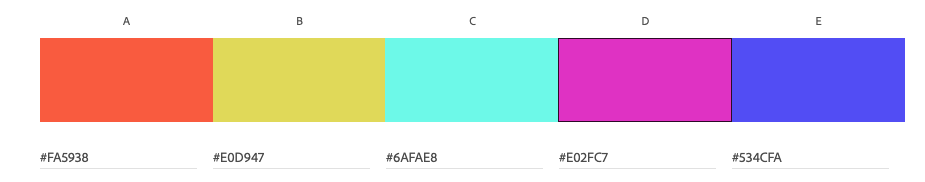
\includegraphics[width=1.0\textwidth]{images/paleta_de_cores_acessiveis.png}
        \caption{Exemplo de uma paleta de cores acessível feita no Adobe Color}
\end{figure}  
 
\vspace*{50px}
É de extrema importância verificar como ficaria essas cores pela visão de pessoas que possuem algum tipo de daltonismo. Ao perceber que a paleta de cores ainda está com um contraste aceitável e de no mínimo 7:1 ela está pronta para o uso. 
 \begin{figure}[ht]
        \centering
    	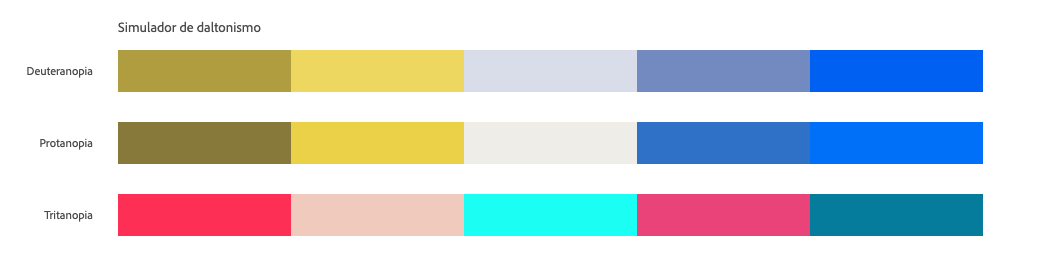
\includegraphics[width=1.0\textwidth]{images/paleta_daltonismo.png}
        \caption{simulação de daltonismo feita no Adobe Color}
\end{figure}  


\newpage
Tipografia: A tipografia não é apenas escolher uma fonte legal para o seu projeto, junto com ela devemos levar em consideração vários aspectos que são importantes e foram listados nas diretrizes: 
\begin{itemize}
\item Espaçamento
\begin{itemize}
\item O espaçamento deve ser bem planejado para que seja possível aplicar um zoom de 200\%\ e ou ainda em caso de redimensionamento de tela o texto deve permanecer legível. 
\end{itemize}
\item Altura de linhas
\begin{itemize}
\item Sempre que houver um redimensionamento os textos não devem perder legibilidade.
\end{itemize}
\item Hierarquia tipográfica
\begin{itemize}
\item Sempre que o conteúdo da tela for dividido em sessões, todas devem possuir títulos claros, com níveis de hierarquia bem definidos, para assim manter a hierarquia da informação de uma forma concisa. 
\end{itemize}
\item Pesos, cores e contraste. 
\begin{itemize}
\item O contraste entre textos e telas também deve ser mantido num padrão de no mínimo 4:5:1
\end{itemize}
\end{itemize}

\begin{figure}[ht]
        \centering
    	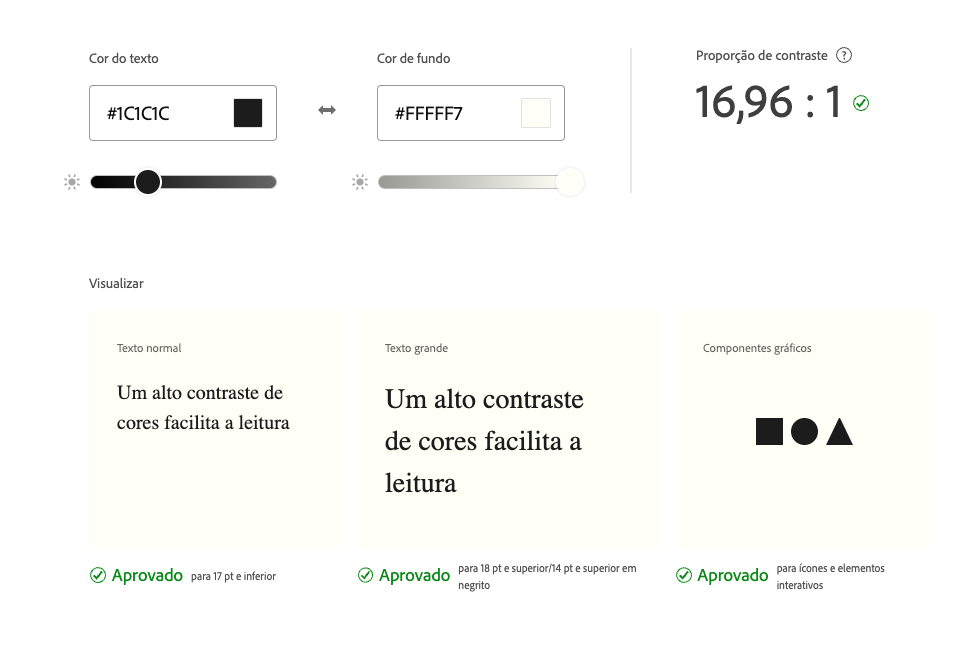
\includegraphics[width=1.0\textwidth]{images/contrast_check.png}
        \caption{Checagem do contraste de textos e fundo no Adobe Color}
\end{figure} 

\newpage
Elementos de UI: Aqui sempre será listado e exemplificado cada elemento que vai compor a UI. Na construção desses elementos é feito o detalhamento visual, ou seja, os tamanhos, espaços, margens, cores que ele deve possuir como também os seus estados comportamentais, se houver um erro como ele se comporta, em caso de elemento focado como deve ficar o elemento.

\begin{wrapfigure}{l}{0.5\textwidth}
        \begin{center}
    	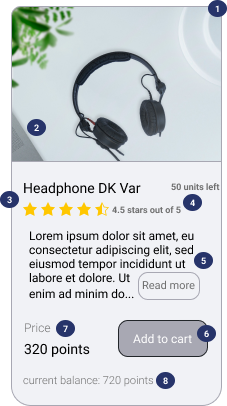
\includegraphics[width=0.48\textwidth]{images/ui-exemplo.png}
        
        \end{center}
        \caption{Exemplo de um componente montado com elementos de UI}
\end{wrapfigure} 

Com o componente Card do exemplo ao lado podemos analisar onde as diretrizes foram aplicadas e como elas impactam na construção de componentes mais complexos de UI. 
\begin{itemize}
\item O elemento sinalizado como 1 está recebendo foco (diretriz 3.2.1 e 2.4.7), a arquitetura desse elemento está fazendo sentido para todos, sejam ouvintes ou leitores (diretriz 1.3.1). A apresentação das informações segue uma sequencia lógica (diretriz 1.3.2).  
\item O número 2 refere-se a imagem onde ela deve ter uma descrição alternativa em texto (diretriz 1.1.1) e deve ter um contraste não textual (diretriz 1.4.11).
\item O terceiro item compreende o cabeçalho do Card. Nesse cabeçalho deve haver um contraste textual de no mínimo (diretriz 1.4.3) e esse cabeçalho deve ser claro o suficiente para a finalidade do conteúdo (diretriz 2.4.6).
\item O quarto item compreende a informações adicionais, sejam elas quantos itens restam disponíveis para compra ou a avaliação daquele item. Para essas informações adicionais além de estarem descritas de forma não "convencional" aos padrões usuais de e-commerce foram aplicadas as diretrizes de contraste textual (diretriz 1.4.11), contraste melhorado (diretriz 1.4.6), etc.
\end{itemize}
\newpage
\begin{itemize}
\item O quinto item é a descrição do produto, essa descrição não está exposta em sua totalidade, para ler o texto completo é necessário apertar o botão para ler mais. Além de todas as diretrizes de contraste que foram aplicadas, está sendo usado as diretrizes de foco (diretrizes 2.4.7 e 3.2.1), o botão presente segue a diretriz de tamanho de área clicável (diretriz 2.5.5), além de ter o nome acessível (diretriz 2.5.3). No botão em questão ainda há o acionamento e foco por teclado (diretrizes 1.4.12, 1.4.13, 2.1.1, 2.1.2 e 2.1.3). 
\item O botão sinalizado pelo número 6 segue as mesmas diretrizes do botão listado no item 5. Além das diretrizes relacionadas a foco (diretriz 2.4.3, 2.4.7), navegação (diretriz 3.2.3, 1.4.12, 1.4.13, 2.1.1, 2.1.2 e 2.1.3), localização (diretriz 2.4.8, 3.2.4) e acionamento (diretriz 2.5.2).
\item O item 7 refere-se a informações sobre preços, onde há um contraste muito nítido para evidenciar a informação mais importante, que no caso é o valor. Nesse item contempla todas as diretrizes de contraste. 
\item O item 8 é uma abordagem diferenciada para informações que são úteis em contextos gerais. Nesse caso é muito atrativo para usuários ouvintes saberem sempre quanto pontos eles dispõem em sua conta, então essa informação está disposta mais facilmente. 
\end{itemize}

}

\subsection{Fase 2: Adaptação e construção da UI acessível e usável usando o guia de acessibilidade e style guide}
{A segunda fase se concentrou na adaptação da UI e na construção de novos componentes para o e-commerce, sempre seguindo os guias. Nessa fase o foco principal se dividiu em três vertentes:
\begin{itemize}
\item Criar abordagens inteligentes para problemas de acessibilidade em imagens, formulários e navegação e a
adaptação de componentes com HTML não semântico para semântico.
\item  Adaptar componentes não semânticos para que as tecnologias assistivas pudessem entendê-los como texto legível e lê-los.
\item  Adaptar componentes não semânticos para que a navegação por teclado fosse eficaz
\end{itemize}
}
\subsubsection{Abordagens inteligentes e adaptação de componentes}
{TODO: colocar exemplos de adaptação de componentes}
\subsubsection{Adaptação de componentes para o uso de leitores de telas}
\subsubsection{Adaptação de componentes para a navegação por teclado}

\subsection{Fase 3: Construção do dashboard acessível}

\subsection{Fase 4: Testes e avaliações de acessibilidade}
{Durante e após a construção do e-commerce de acordo com os
padrões Web e as diretrizes de acessibilidade, é necessário efetuar testes para garantir sua acessibilidade. Esses testes foram executados de dois modos: 
\begin{itemize}
\item Avaliação automática: São as avaliações feitas de maneira automática por meio de plugins de verificação e de websites de validação.
\begin{itemize}
\item Google Accessibility Developer Tools (Plugin para navegador Chrome)
\item Axe DevTools 
\item Accessibility Engine (axe) (Plugin para navegador Chrome e Firefox)
\item Contrast Checker (website - Validação de contraste de cores
\end{itemize}
\item Avaliações manuais: Essa etapa pode ser feita usando o leitor de tela e a navegação por teclado, onde deve ser checado se todos os comportamentos e ações esperados estão sendo realmente respeitados e executados. 

\end{itemize}
}

\subsection{Tecnologias utilizadas} 
{A linguagem de programação JavaScript foi escolhida para a elaboração deste trabalho devido a sua grande relevância no frontend. Entre as principais bibliotecas utilizadas neste projeto destaca-se:
\begin{itemize}
\item React.js
\item HTML
\item Sass
\item D3.js
\item Diretrizes WCAG
\item WAI-ARIA
\item Tecnologias assistivas:
\begin{itemize}
\item VoiceOver
\item NVDA
\item ORCA
\end{itemize}
\end{itemize}
 
\subsection{Contribuição}
\textcolor{violet}{A sua contribuição já encontra-se no ambiente de produção? Há quanto tempo? Qual é a sua percepção sobre o impacto da sua contribuição na empresa?}
{⁠A solução ainda não se encontra em produção, pois está passando por um processo de alinhamento sobre outros pontos que o cliente deseja modificar dentro do sistema. 

Esse projeto e tudo construído nele se tornou um tipo de referência para outros desenvolvedores e designers que buscam aprender mais sobre a acessibilidade e aplicá-la de um modo descomplicado e correto, o guia está sendo construído justamente com a intenção de ser um objeto compartilhado pelos desenvolvedores do CESAR e servir como orientação para todos. 
 }
